\chapter{Campioni chirurgici}

\section{Introduzione ai pezzi chirurgici}
I campioni chirurgici rispetto alle piccole biopsie e alle cuti spesso richiedono una descrizione macroscopica più elaborata e un camionamento selettivo, pertanto l'esame macroscopico ed il campionamento richiedono che siano chiari quali siano gli elementi necessari per la formulazione della diagnosi patologica.

\subsection{La chirurgia elettiva}
Un paziente generalmente va incontro a chirurgia in due situazioni principali. La prima riguarda le chirurgie elettive, ovvero quelle pianificate, in cui c'è una diagnosi o un sospetto diagnostico molto forte che giustifica l’intervento chirurgico. Questo tipo di intervento ha lo scopo di rimuovere un processo patologico, che può essere di natura neoplastica o infiammatoria. Nel caso della chirurgia elettiva, tutto è programmato: il paziente si sottopone all’intervento sulla base di un sospetto diagnostico o di una diagnosi istologica precedente.

\subsection{La chirurgia non elettiva}
La seconda situazione è la chirurgia non elettiva, ovvero un intervento d'urgenza. Questi casi si presentano in varie circostanze, come traumi o, più comunemente in anatomia patologica, perforazioni di visceri. Ad esempio, una perforazione intestinale può derivare dall'ingestione di materiale estraneo o da patologie infiammatorie. In questa categoria, i campioni più frequenti sono quelli derivanti da chirurgie generali, come le appendiciti acute, sebbene oggi si preferisca spesso il trattamento con antibiotici. Altri esempi possono includere perforazioni intestinali o infarti intestinali causati da processi come l'intussuscezione, in cui un segmento dell'intestino si invagina su se stesso, fenomeno associato a masse della parete, soprattutto negli adulti.

\subsection{Finalità del campionamento}
Il campionamento dei pezzi operatori è finalizzato alla formulazione di una diagnosi. Per le patologie neoplastiche, la diagnosi non si limita all'identificazione del tipo di tumore, ma cerca anche di fornire informazioni utili ai vari specialisti che si occupano del paziente oncologico, come oncologi, radioterapisti e chirurghi. Questo approccio è particolarmente importante per identificare i cosiddetti parametri \textit{prognostici} e \textit{predittivi}.\footnote{I parametri \textit{prognostici} forniscono informazioni sul probabile decorso della malattia, indipendentemente dal trattamento. In altre parole, aiutano a prevedere come si comporterà la patologia nel tempo. I parametri \textit{predittivi}, invece, indicano la probabile risposta a un determinato trattamento, aiutando a scegliere la terapia più efficace.} Per quanto riguarda i campioni di chirurgia non elettiva, l'obiettivo è capire il motivo dell'evento acuto o emergente che ha richiesto l'intervento. Anche qui, il fine è quello di formulare una diagnosi precisa. Questo è il motivo per cui il campione viene inviato in anatomia patologica: fornire una risposta che possa guidare la gestione clinica successiva.

\subsection{Apertura del pezzo chirurgico}
I campioni chirurgici, rispetto ai campioni bioptici o di piccole dimensioni, richiedono una cura particolare, soprattutto se il campionamento non viene eseguito tempestivamente dopo il prelievo. In questi casi, il rischio principale è l’autolisi o la sovrainfezione da muffe e batteri presenti sul campione. Per evitare tali complicazioni, si effettua l'apertura del pezzo. Il primo passo, quando il campione arriva in anatomia patologica, consiste nel sezionare il pezzo (se composto da parenchimi) o nell’aprire eventuali cavità, per permettere la penetrazione uniforme della formalina in tutto il campione. La formalina ha la funzione di bloccare tutti i processi biologici, sia quelli interni al campione che quelli derivanti da contaminazioni esterne. Questo procedimento è essenziale per garantire una fissazione omogenea, il che a sua volta assicura una buona immunoreattività del campione, come discusso nel capitolo dedicato alla fissazione.

\subsection{Orientamento del pezzo chirurgico}
Infine, oltre alla sfida del campionamento e della selezione del materiale che sarà processato per ottenere i vetrini, i campioni chirurgici pongono un ulteriore problema: l'orientamento del pezzo anatomico. Ma cosa significa orientare un pezzo chirurgico? Orientare un pezzo chirurgico significa documentare la sua disposizione tridimensionale e identificare con precisione la localizzazione delle strutture anatomiche importanti, come i margini di resezione. Questo passaggio è fondamentale poiché permette di fornire informazioni corrette su eventuali infiltrazioni neoplastiche e su altre caratteristiche rilevanti per la diagnosi e la stadiazione del tumore. Nel prossimo paragrafo vedremo come il campionamento debba tenere conto di questi aspetti per garantire una corretta interpretazione dei risultati da parte del patologo.

\section{Distinzione fra pezzi neoplastici e non neoplastici}

\subsection{Cos'è una neoplasia}
Il termine \textit{neoplasia} deriva dal greco, con il prefisso \textit{neo-} che significa "nuovo" e \textit{plazo} che significa "crescere". Analogamente, in latino, il termine \textit{tumor} si riferisce a un "gonfiore". Entrambi i termini, nel loro significato originario, indicano un processo di crescita anomala che non fa parte della normale anatomia. In epoca moderna, il termine \textit{neoplasia} è usato per indicare un processo cellulare caratterizzato da una proliferazione di cellule anomale che crescono in maniera incontrollata. La neoplasia rappresenta quindi una crescita cellulare fuori dal controllo dei normali meccanismi di omeostasi cellulare.\footnote{In passato, il termine \textit{tumore} era utilizzato per indicare qualsiasi gonfiore anomalo, mentre oggi si riferisce esclusivamente alla proliferazione clonale di cellule mutate, che hanno perso il controllo della crescita. Questo concetto è cruciale per comprendere le malattie neoplastiche.}

\subsection{Caratteristiche delle neoplasie}
Le malattie neoplastiche si presentano, dal punto di vista macroscopico, come masse o crescite anomale all'interno di un tessuto. Per identificare una neoplasia, è necessario avere una profonda conoscenza dell'anatomia normale, poiché l’aspetto macroscopico del campione patologico si confronta sempre con ciò che è considerato normale. Le neoplasie possono manifestarsi in modi diversi: all'interno dei parenchimi come masse che crescono in modo espansivo nelle tre dimensioni, oppure negli organi cavi come una crescita superficiale che si espande progressivamente verso strati più profondi con l'aggressività della neoplasia. Durante il campionamento, è essenziale prestare attenzione anche alle piccole masse, spesso non evidenziate dal chirurgo, poiché in anatomia patologica si ha la responsabilità finale di fornire una diagnosi definitiva.

\subsection{Sierosite}
Le patologie infiammatorie e non neoplastiche si distinguono macroscopicamente da quelle neoplastiche per alcuni aspetti caratteristici. Uno dei segni principali dell'infiammazione è l'opacizzazione delle sierose. Questo fenomeno è spesso osservato in patologie come l'appendicite o le malattie infiammatorie croniche intestinali. Le sierose, come il peritoneo, che normalmente sono lucide, diventano opache e possono essere ricoperte da un induito fibrinoso, ovvero un sottile strato biancastro di fibrina.

\subsection{Infiammazione}
In anatomia patologica, la descrizione macroscopica dell'infiammazione segue i criteri classici di Virchow: \textit{tumor} (gonfiore), \textit{rubor} (rossore), \textit{calor} (calore), \textit{dolor} (dolore) e \textit{functio laesa} (alterazione della funzione). Sebbene non siano tutti apprezzabili macroscopicamente  gonfiore (tumor) e arrossamento (rubor) sono visibili e utilizzati per identificare processi infiammatori. Ad esempio, in un caso di appendicite acuta, l'appendice appare edematosa, rigonfia e arrossata, e può presentare materiale purulento (raccolta di pus). Questo materiale purulento corrisponde, al microscopio, a un infiltrato di neutrofili e tessuto di granulazione. Quando si verificano raccolte più significative di pus, si può parlare di ascessi.

\subsection{Fibrosi e granulomi}
Un altro segno caratteristico di patologie non neoplastiche è la presenza di fibrosi, che distorce l'anatomia normale e può rendere difficile distinguere queste lesioni da masse neoplastiche. Un altro processo che spesso entra in diagnosi differenziale (ovvero si può confondere) con una lesione neoplastica è rappresentato dalle infezioni croniche sostenute da micobatteri o funghi, che possono causare la formazione di granulomi. Queste lesioni possono creare difficoltà diagnostiche, tanto che noduli polmonari non diagnosticati durante biopsie spesso possono essere analizzati in estemporanea dove viene fatta diagnosi di flogosi granulomatosa gigantocellulare con necrosi caseosa (il quadro morfologico della tubercolosi).

\subsection{Campionamento dell'alterazione macroscopica}
In conclusione, i pezzi neoplastici e non neoplastici spesso si distinguono chiaramente dal punto di vista macroscopico. Le neoplasie si presentano come crescite anomale e disorganizzate, spesso di natura espansiva o infiltrativa, mentre le patologie infiammatorie non neoplastiche sono caratterizzate da segni di infiammazione, fibrosi e talvolta raccolte di materiale purulento. La corretta identificazione di questi elementi macroscopici è fondamentale per identificare quali campioni scegliere per la microscopia, e in generale vale la regola in patologia chirurgica che tutte le alterazioni macroscopiche vanno confermate itologicamente.

\section{Campioni neoplastici}

\subsection{Impatto della diagnosi patologica}
La descrizione macroscopica dei campioni neoplastici è cruciale per comprendere la natura e l'estensione del processo patologico. Il referto anatomopatologico rappresenta il documento su cui si basa la gestione futura del paziente oncologico, sia che si tratti di una diagnosi iniziale, sia di una recidiva o di una metastasectomia. Le decisioni cliniche e terapeutiche dipendono strettamente dalle informazioni fornite nel referto.

\subsubsection{Istotipo e Grado}
Il referto anatomopatologico di un pezzo chirurgico è fondamentale nella gestione del paziente oncologico. Esso fornisce una diagnosi definitiva, indicando l’istotipo del tumore e stabilendo il grado di aggressività sulla base di parametri biologici. In particolare, il grado di un tumore descrive quanto esso perde somiglianza rispetto al tessuto di origine.

Ogni tipo di tumore ha il suo sistema di gradazione. Ecco alcuni esempi:
\begin{itemize}
    \item \textbf{Carcinoma spinocellulare:} Il sistema di \textit{Broder} valuta quanto il tumore si differenzia dall'epitelio spinocellulare normale.
    \item \textbf{Carcinoma mammario:} Il grading di \textit{Elston-Ellis} si basa sulla formazione di dotti, il numero di mitosi e il pleomorfismo.
    \item \textbf{Carcinoma della prostata:} Il sistema di \textit{Gleason} valuta l'architettura delle cellule neoplastiche all'interno della prostata.
    \item \textbf{Carcinoma del polmone:} Il carcinoma spinocellulare del polmone segue il grading di Broder, mentre  l'adenocarcinoma polmonare (che oggi rappresenta l'istotipo più frequente) varia in base al sottotipo istologico: i tumori con crescita lepidica sono di grado 1, con crescita acinare o papillare sono di grado 2, mentre quelli con crescita solida o micropapillare sono di grado 3.
\end{itemize}

\begin{figure}[p]
    \centering
    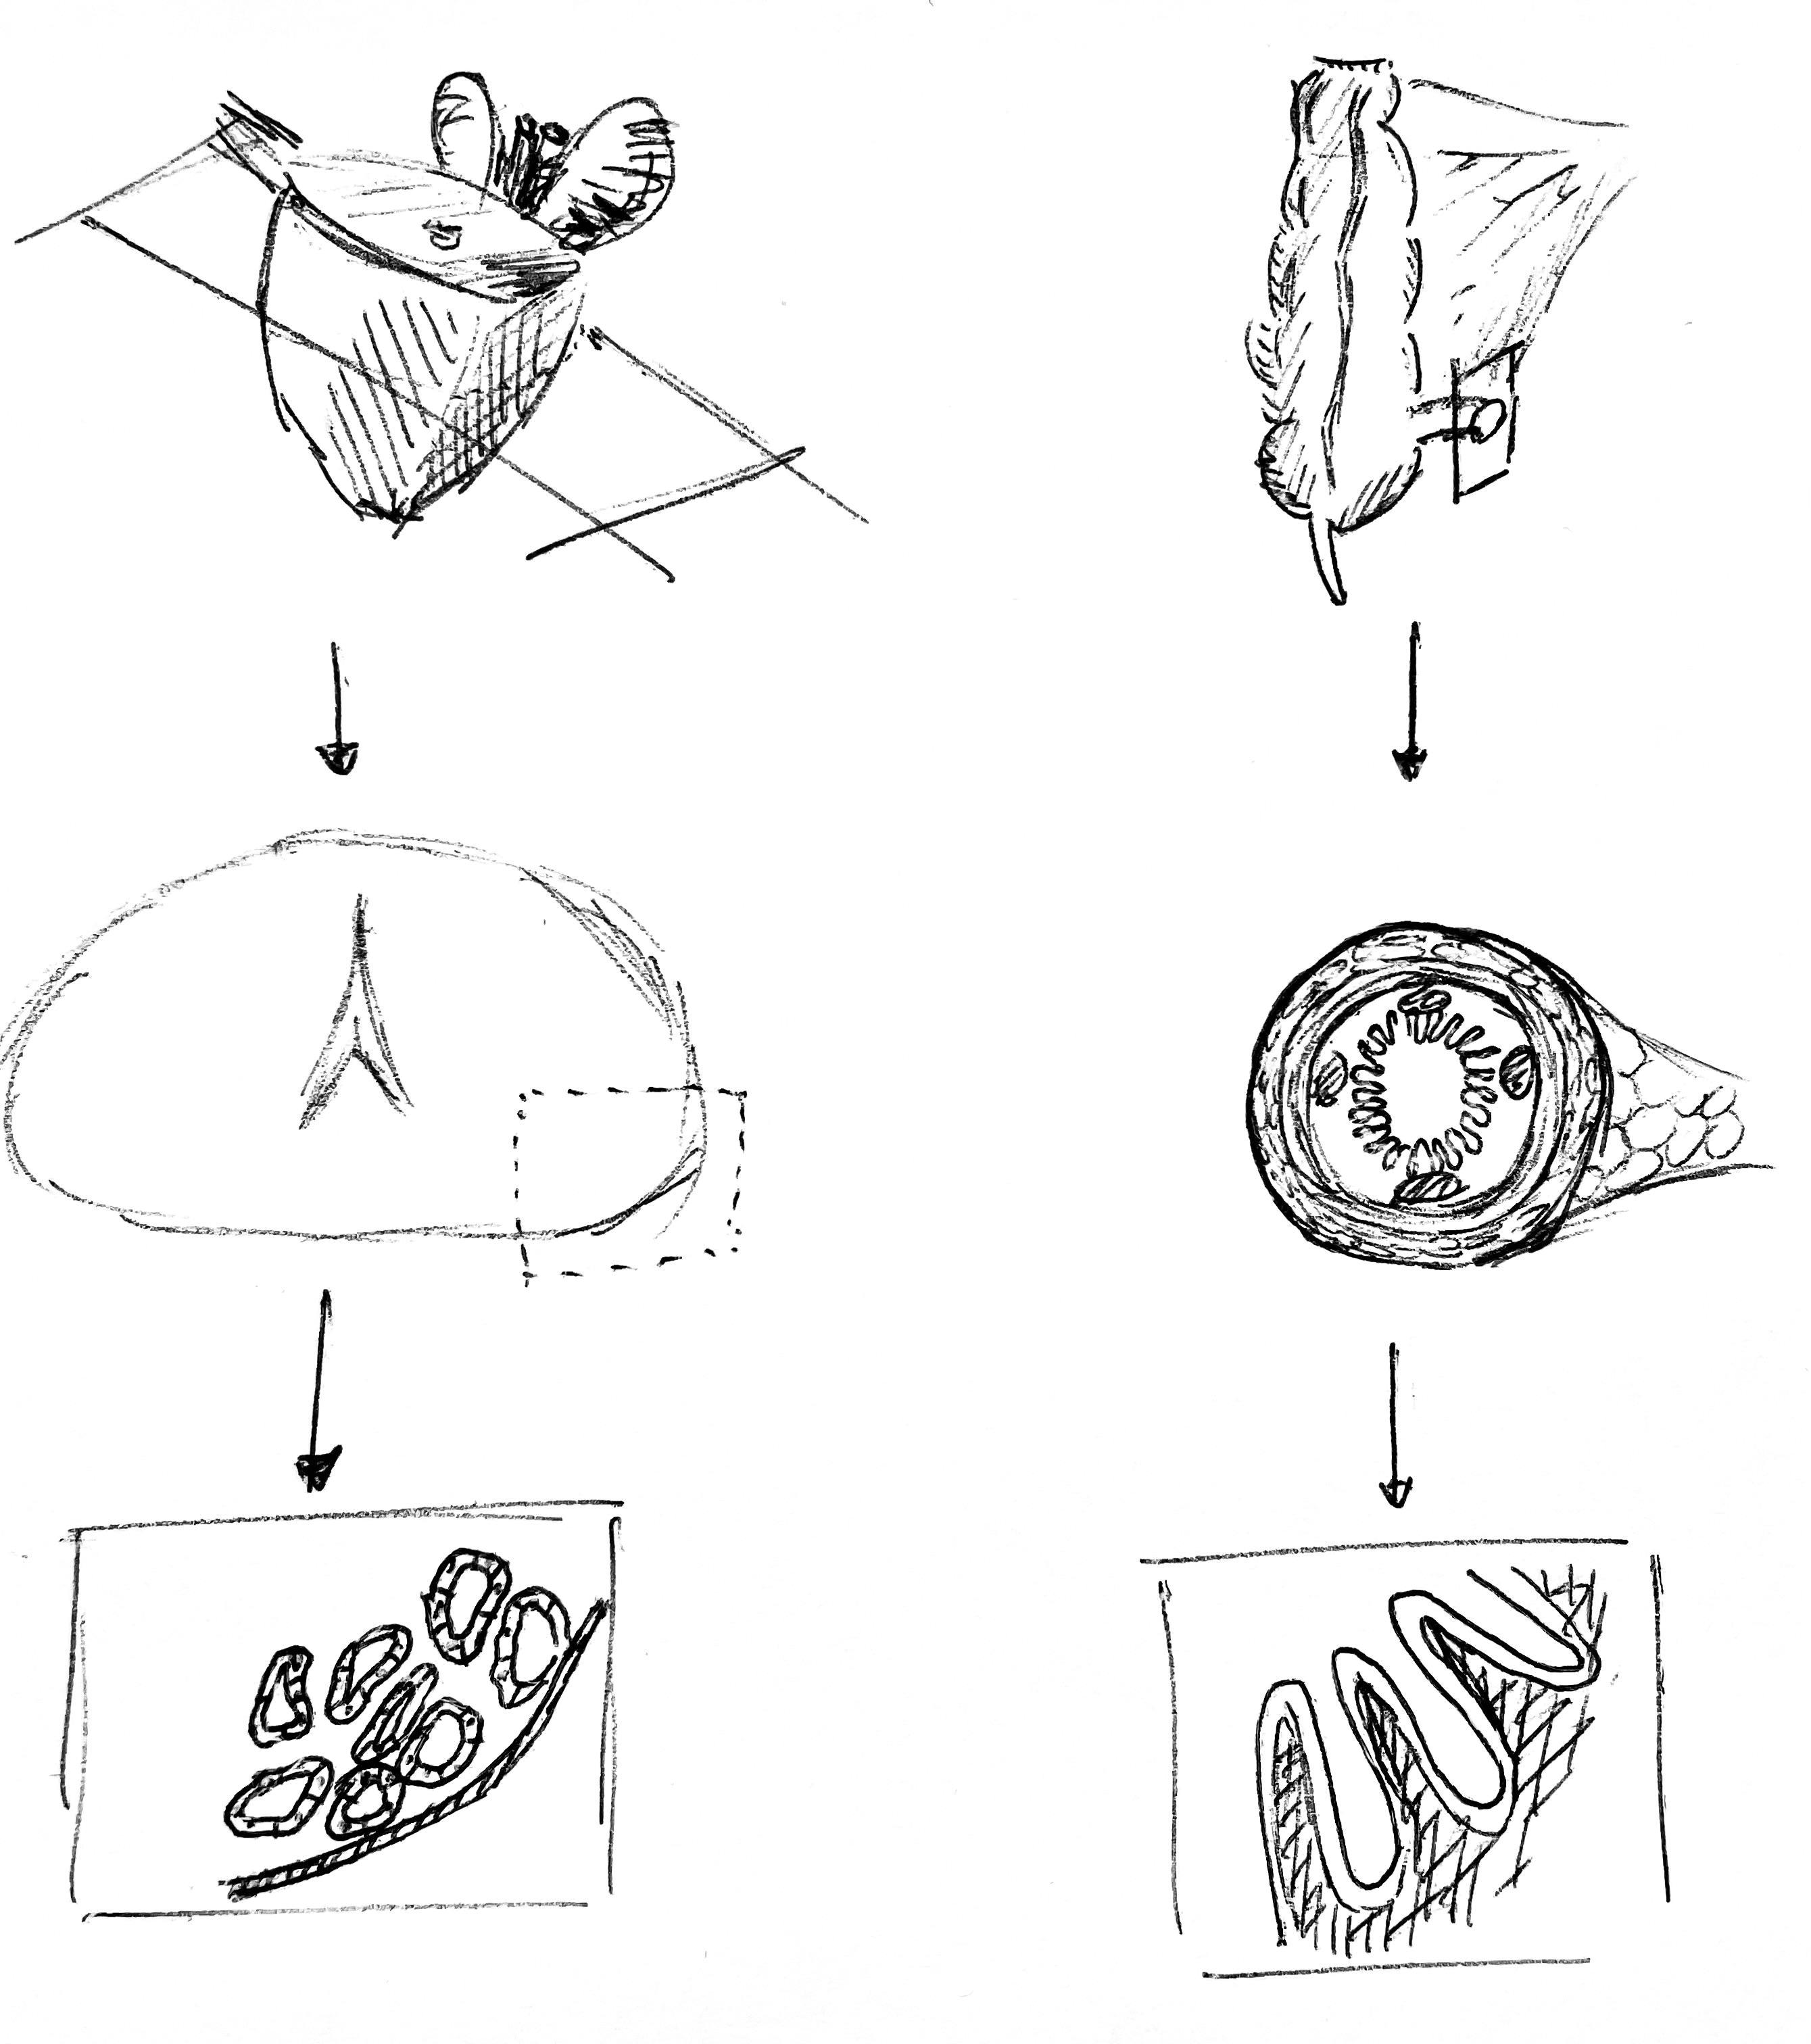
\includegraphics[width=0.75\textwidth]{campionamento_margini}
    \caption{Il campionamento margini}
    \label{fig:campionamento_margini}
\end{figure}

\subsection{Valutazione dei margini chirurgici}
Un elemento fondamentale del referto è la valutazione dei margini chirurgici, che indicano la fine del pezzo anatomico e l'inizio del tessuto sano. I margini possono essere campionati in modi diversi (Figura \ref{fig:campionamento_margini}):
\begin{itemize}
    \item \textbf{Margini campionati con inchiostro:} L'inchiostro di china viene applicato per evidenziare il margine anatomico. Se il tumore si trova su questa linea colorata, il margine è considerato positivo (\textit{tumor on ink}).
    \item \textbf{Margini campionati \textit{en face}:} Per organi cavi, il margine viene incluso sul versante che rappresenta il margine anatomico. In questo caso, se vi è tumore sul margine \textit{en face}, il margine è coinvolto.
\end{itemize}

La valutazione dei margini varia a seconda del tipo di tumore. Ad esempio, nel tumore della prostata, la presenza di tumore sulla china indica un margine positivo. In altri casi, una semplice vicinanza del tumore al margine può bastare per stabilire una non radicalità oncologica.

Il sistema di radicalità chirurgica prevede tre livelli:
\begin{itemize}
    \item \textbf{R0:} Radicalità microscopica, ovvero assenza di tumore sui margini.
    \item \textbf{R1:} Positività microscopica del margine.
    \item \textbf{R2:} Positività macroscopica, indicante che il chirurgo non è riuscito a ottenere una radicalità chirurgica completa.
\end{itemize}

\subsection{Stadiazione TNM}
La stadiazione è un altro aspetto critico della valutazione anatomopatologica. Il sistema più utilizzato è il \textit{TNM}, adottato da organizzazioni internazionali come l'UICC (Unione Internazionale Contro il Cancro) e l'AJCC (American Joint Committee on Cancer). Il sistema valuta tre parametri:
\begin{itemize}
    \item \textbf{T:} Dimensioni e estensione del tumore primitivo.
    \item \textbf{N:} Coinvolgimento dei linfonodi (nodes).
    \item \textbf{M:} Presenza di metastasi a distanza.
\end{itemize}

Il patologo è responsabile della stadiazione patologica (\textit{pTNM}), che si differenzia dalla stadiazione clinica (\textit{cTNM}) utilizzata per la diagnosi pre-operatoria. Ogni neoplasia ha un suo sistema di stadiazione TNM. Di seguito, riportiamo una tabella comparativa del sistema TNM per il tumore della mammella e per il tumore del colon:

\begin{table}[h!]
    \centering
    \begin{tabular}{|c|c|c|}
        \hline
        \textbf{Stadio} & \textbf{TNM Mammella} & \textbf{TNM Colon} \\
        \hline
        T1 & Tumore \textless 2 cm & Tumore invade la sottomucosa \\
        \hline
        T2 & Tumore 2-5 cm & Tumore invade la muscolare propria \\
        \hline
        T3 & Tumore \textgreater 5 cm & Tumore invade la sierosa \\
        \hline
        N1 & 1-3 linfonodi coinvolti & 1-3 linfonodi regionali coinvolti \\
        \hline
        N2 & 4-9 linfonodi coinvolti & 4-6 linfonodi regionali coinvolti \\
        \hline
        M1 & Metastasi a distanza presenti & Metastasi a distanza presenti \\
        \hline
    \end{tabular}
    \caption{Confronto tra il sistema TNM della mammella e del colon}
    \label{tab:tnm_comparativo}
\end{table}

\subsection{Importanza del campionamento nella patologie neoplstiche}
Il referto anatomopatologico e la descrizione macroscopica sono essenziali per la diagnosi, la valutazione dei margini e la stadiazione di ogni tumore. Questi elementi determinano il trattamento e la gestione clinica del paziente oncologico, influenzando direttamente il successo terapeutico.

\section{Tumore della mammella}
Le resezioni di mammella per carcinoma rappresentano uno dei campioni chirurgici più frequenti in anatomia patologica, riflettendo la sua alta incidenza nell'epidemiologia oncologica. I campioni derivanti da interventi chirurgici possono essere di diversi tipi, inclusi quadrantectomie, nodulectomie, mastectomie radicali o mastectomie sottocutanee con risparmio del capezzolo. Ogni procedura ha lo scopo di rimuovere il tessuto mammario contenente la neoplasia, che nella maggior parte dei casi è un carcinoma. Gli istotipi più prevalenti sono il \textit{carcinoma istotipo non speciale} e il \textit{carcinoma lobulare}.

Questi due istotipi sono importanti perché la presentazione macroscopica e le modalità di campionamento possono variare significativamente.

\subsection{Strategie di campionamento}
Per una corretta valutazione, è essenziale applicare le corrette strategie di campionamento, che variano a seconda del tipo di intervento chirurgico e delle dimensioni del tumore.

\subsection{Quadrantectomia}
Le quadrantectomie sono solitamente eseguite per tumori di piccole dimensioni, spesso inferiori a 2 cm. Il chirurgo orienta il pezzo tramite fili di repere e, in alcuni casi, include la cute per aiutare l'anatomopatologo a identificare i margini. Questo tipo di campione viene frequentemente inviato per esame intraoperatorio, con l’obiettivo di valutare la distanza del tumore dai margini chirurgici (Figura \ref{fig:campionamento_mammella}).

Il campionamento macroscopico avviene dopo la marcatura della superficie esterna del campione con inchiostro di china. Successivamente, il quadrante viene sezionato con tagli sottili, generalmente con uno spessore massimo di 5 mm, per permettere una chiara identificazione anche di piccoli noduli. Spessori superiori potrebbero impedire l’identificazione di neoplasie più piccole, compromettendo la diagnosi.


\begin{figure}[p]
    \centering
    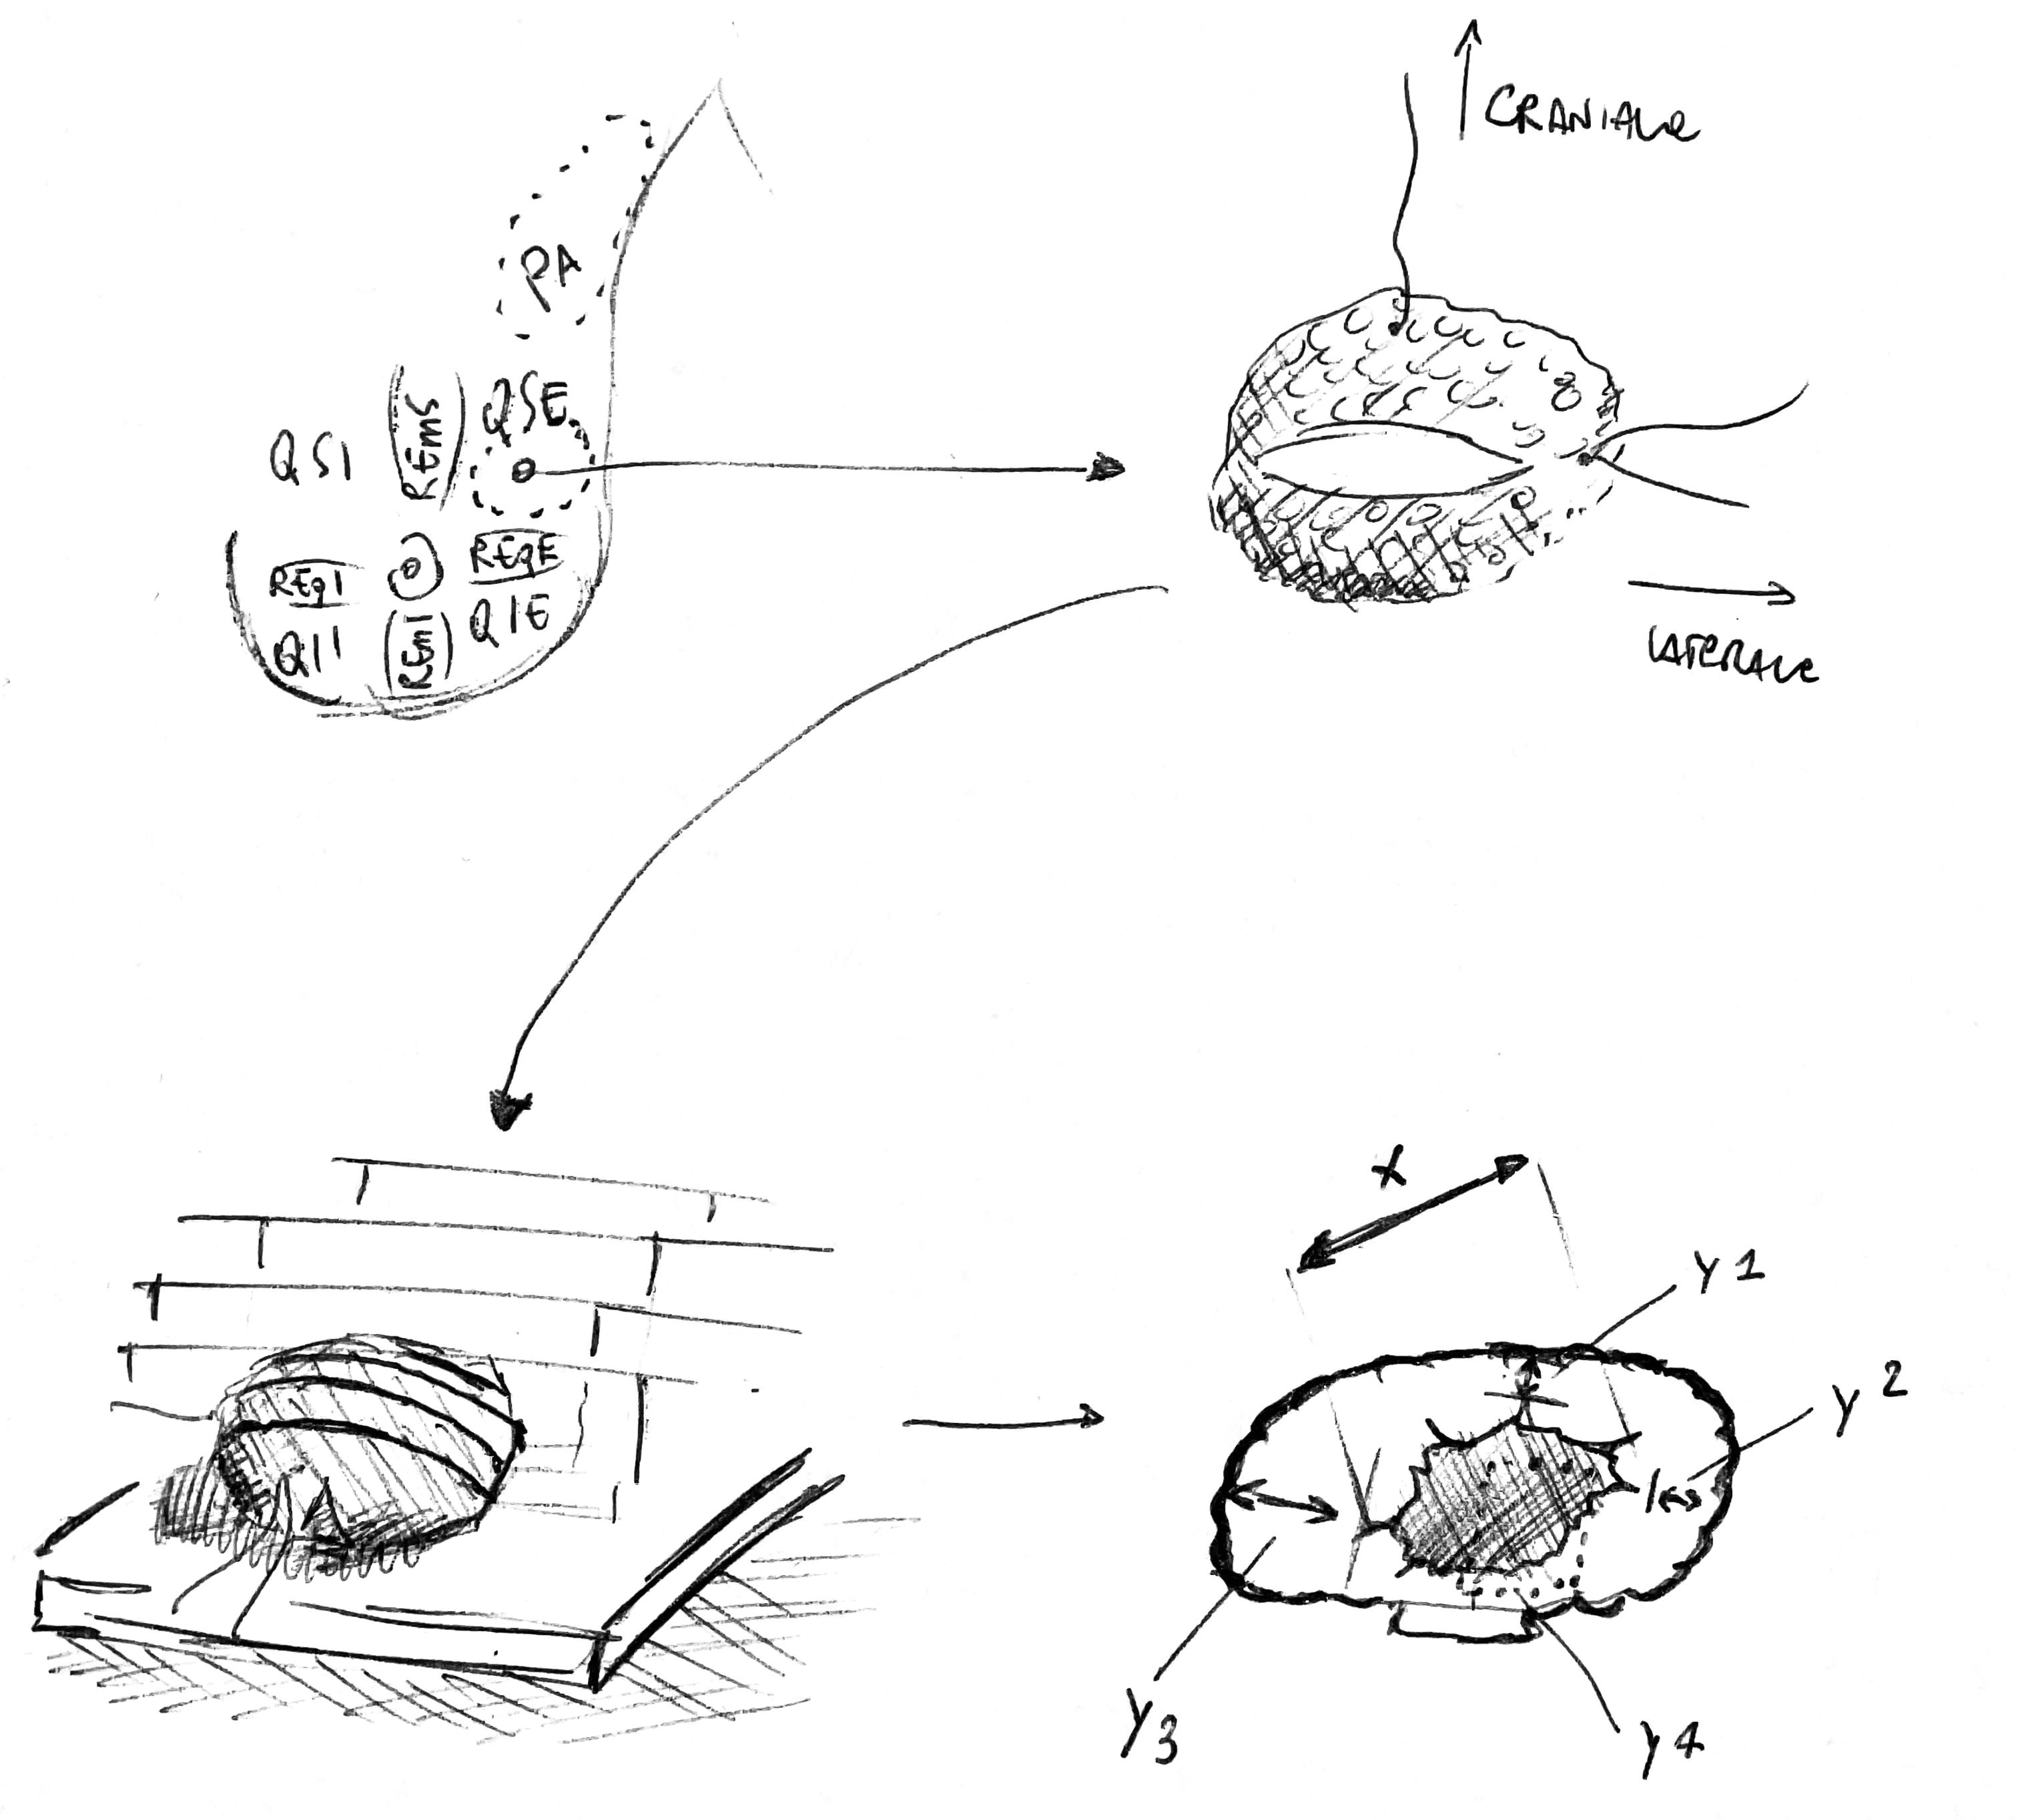
\includegraphics[width=0.755\textwidth]{campionamento_mammella}
    \caption{Il campionamento della quadrantectomia.  La mammella (figura in alto a sinistra) viene divisa in quattro quadranti: supero esterno (QSE), infero esterno (QIE), infero interno (QII) e supero interno (QSI); inoltre si identificano le regioni equatoriale esterna (REqE) ed interna (REqI) ed emitelica superiore (REmS) ed inferiore (REmI); ed infine il prolungamento ascellare (PA) e la regione retroareolare. Oggi la quadrantectomia è spesso una nodulectomia che rimuove solo parte del quadrante e arriva in anatomia patologica orientata da fili di repere (figura in alto a destra) che permettono al patologo di poter ricostruire la distanza dei margini dalla neoplasia. Il campione viene chinato e sezionato con delle sezioni di 4-5 mm di spessore (figura in basso a sinistra) e macroscopicamente si misurano (figura in basso a destra) il diametro massimo del tumore (x) e la distanza da tutti margini (y).}
    \label{fig:campionamento_mammella}
\end{figure}

\subsection{Mastectomia}
Le mastectomie, eseguite per tumori di dimensioni maggiori o per indicazioni oncologiche specifiche, richiedono una strategia di campionamento più estesa. Il piano profondo del campione viene marcato con china e il pezzo viene orientato, identificando in quali quadranti si trovano le neoplasie. Anche in questo caso, il tessuto viene sezionato ogni 5 mm per garantire l’identificazione di eventuali masse tumorali nascoste.

Quando sono presenti più neoplasie, è essenziale campionare accuratamente il tessuto interposto tra i vari tumori per determinare se queste lesioni sono indipendenti o connesse tra loro. Due masse macroscopicamente separate potrebbero risultare parte della stessa neoplasia quando osservate al microscopio. Pertanto, è importante misurare le dimensioni di ciascun tumore e della massa complessiva nel caso di una singola neoplasia con tessuto interposto coinvolto.

\subsubsection{Misurazione dei margini chirurgici}
Uno degli obiettivi principali dell’esame macroscopico è determinare la distanza tra la neoplasia e i margini chirurgici, elemento fondamentale per la valutazione della radicalità dell’intervento. Nel caso di una quadrantectomia, il margine può essere valutato sia macroscopicamente che intraoperatoriamente, mentre nelle mastectomie l’intero tessuto asportato viene campionato per garantire un’adeguata valutazione dei margini.

\subsubsection{Fattori prognostici e predittivi}
Nel tumore della mammella, oltre alla dimensione e alla diffusione del tumore, il referto anatomopatologico deve includere i cosiddetti fattori prognostico-predittivi. Questi comprendono:
\begin{itemize}
    \item Il recettore per l'estrogeno (ER)
    \item Il recettore per il progesterone (PR)
    \item L’\textit{HER2/neu}
    \item Il \textit{Ki-67}, un marker di proliferazione cellulare.
\end{itemize}

Queste analisi vengono eseguite sul campione operatorio e sono cruciali per determinare il trattamento successivo, inclusa l’idoneità a terapie ormonali o mirate. Il campione prelevato al banco deve includere l'interfaccia tra il tumore e il tessuto mammario normale, per permettere un controllo interno adeguato delle reazioni immunoistochimiche.

\subsubsection{Conclusione}
La gestione dei campioni chirurgici del tumore della mammella richiede una meticolosa attenzione alla tecnica di campionamento e alla misurazione dei margini chirurgici. Un campionamento appropriato garantisce non solo una diagnosi accurata, ma fornisce anche le informazioni necessarie per la stadiazione del tumore e la determinazione dei fattori prognostici e predittivi essenziali per la gestione clinica del paziente.

\section{Tumore del polmone}
Il tumore del polmone, rispetto ad altre neoplasie cosiddette \textit{Big Killers}, tende a presentarsi in stadi più avanzati e presenta delle peculiarità per quanto riguarda la stadiazione e il campionamento anatomopatologico. L'istotipo più frequente è l'adenocarcinoma, seguito dal carcinoma spinocellulare e, più raramente, dal carcinoma a piccole cellule.

\subsection{Caratteristiche istologiche e distribuzione}
L'adenocarcinoma del polmone si localizza prevalentemente nelle porzioni periferiche del parenchima polmonare, spesso in prossimità della pleura. Questa caratteristica rende frequente l'infiltrazione pleurica, un parametro cruciale per la stadiazione del tumore polmonare. Il carcinoma spinocellulare e il carcinoma a piccole cellule, invece, tendono a svilupparsi in sede centrale, spesso lungo l'albero bronchiale principale. In particolare, il carcinoma spinocellulare può causare occlusione bronchiale, determinando un'atelettasia del tessuto polmonare distale\footnote{L'atelettasia è il collasso parziale o totale del tessuto polmonare, che può avvenire a causa dell'ostruzione di un bronco da parte di un tumore o di un altro fattore.}. Anche questa condizione è rilevante per la stadiazione, così come la presenza di infiltrazione linfonodale, frequente nei tumori centrali.

\subsection{Approccio al campione chirurgico}
Il campione chirurgico può derivare da una \textit{resezione polmonare tipica} (lobectomia) o da una pneumonectomia. In generale, tali resezioni sono eseguite per adenocarcinomi e altre neoplasie polmonari. Nelle resezioni polmonari tipiche, si seziona la neoplasia insieme al tessuto circostante per garantire una corretta valutazione. Prima di sezionare il pezzo, si rimuove il margine chirurgico, spesso rappresentato da una suturatrice meccanica (\textit{stapler}), che utilizza graffette metalliche per chiudere il tessuto. Le graffette vengono rimosse, ma il vero margine chirurgico sarà valutato solo se il margine parenchimale risulta positivo. 

Il campione viene quindi sezionato in fette sottili, e si cerca il tumore, caratterizzato da una consistenza più dura rispetto al parenchima polmonare circostante, che risulta morbido. Un campionamento abbondante è raccomandato, con un prelievo per ogni centimetro di neoplasia, in quanto il grado istologico del tumore è un parametro cruciale. Vengono inoltre campionate le aree macroscopicamente disomogenee e le eventuali interazioni con la pleura.

\subsection{Campionamento dell’albero bronchiale}
Nelle resezioni lobari e nelle pneumonectomie, si campiona anche il margine dell'albero bronchiale. Dopo l’apertura del bronco con delle forbici, si cercano linfonodi lungo le diramazioni bronchiali, i quali sono rilevanti per la stadiazione linfonodale.

\subsubsection{Carcinoma spinocellulare}
Nel carcinoma spinocellulare, che origina dall'epitelio bronchiale, è essenziale campionare accuratamente il bronco per dimostrare l'infiltrazione tumorale. È importante misurare la distanza del tumore dal margine bronchiale per valutare la radicalità chirurgica.

\subsubsection{Valutazione dei linfonodi}
Il patologo deve campionare accuratamente i linfonodi sia in prossimità del tumore (N1) che nei livelli linfonodali più centrali (N2). I linfonodi inviati dal chirurgo durante l'intervento sono generalmente indicatori di uno stadio linfonodale avanzato (N2 o superiore), mentre i linfonodi recuperati direttamente dal campione chirurgico appartengono solitamente al livello N1.

\subsubsection{Conclusione}
La gestione dei campioni chirurgici del tumore del polmone richiede una valutazione meticolosa per determinare la presenza di infiltrazione pleurica, la distanza dai margini bronchiali e la stadiazione linfonodale. Questi parametri influenzano significativamente la prognosi e la scelta terapeutica per il paziente affetto da tumore polmonare.

\section{Tumore del colon-retto}
Il tumore del colon presenta due tipologie di resezioni chirurgiche più frequenti: la \textit{emicolectomia destra} e la \textit{resezione sigma-rettale}, che può essere più o meno estesa, comprendendo anche il retto. In quest'ultimo caso, si parla di \textit{resezione anteriore} del retto.

Il carcinoma del colon-retto è un \textit{adenocarcinoma} che origina dall'epitelio ghiandolare del rivestimento colico e che progressivamente invade i vari strati della parete del viscere: mucosa, sottomucosa, muscolare propria e tessuto adiposo fino alla tonaca sierosa, che rappresenta lo stadio più avanzato.

\subsection{Resezione anteriore del retto}
Nel caso della resezione anteriore del retto, particolare attenzione va posta alla qualità della resezione chirurgica, poiché il retto non è una struttura peritonizzata e non presenta quindi una superficie sierosa che limiti l'espansione tumorale. La continuità della superficie di resezione è un parametro cruciale per valutare la radicalità chirurgica. Se la superficie risulta discontinua, si parla di \textit{resezione non radicale}, con implicazioni importanti sulla prognosi del paziente.

\subsubsection{Terapia neoadiuvante}
I campioni chirurgici del colon, soprattutto nel caso di neoplasie del retto, possono derivare da interventi eseguiti dopo terapia neoadiuvante. In questi casi, il tumore può risultare difficile da valutare a causa di modificazioni indotte dalla terapia stessa. Un campionamento esteso è raccomandato. 

Il carcinoma può presentarsi sotto diverse forme macroscopiche:
\begin{itemize}
    \item \textit{Polipoide o sessile}: la neoplasia si proietta nel lume intestinale.
    \item \textit{Piatta}: la neoplasia non si proietta nel lume e può infiltrare la parete senza alterare significativamente la sua superficie.
    \item \textit{Ulcerata}: con formazione di una perdita di sostanza nella parete del viscere.
\end{itemize}

Il campionamento del pezzo consiste nel sezionare il colon e identificare il punto di massima infiltrazione tumorale, campionando la sezione con la maggiore invasione degli strati della parete intestinale, soprattutto a livello della muscolare propria.

Analogamente al tumore della mammella, spesso viene eseguita la valutazione delle proteine del \textit{mismatch repair} (MMR)\footnote{Le proteine del \textit{mismatch repair} (MMR) sono coinvolte nella riparazione degli errori di appaiamento del DNA. L'assenza di queste proteine causa instabilità microsatellitare (MSI), un'alterazione molecolare presente in una quota di carcinomi del colon-retto, associata a una migliore prognosi e alla risposta alla terapia con inibitori del checkpoint immunitario.}. 

È necessario che il campione contenga un'interfaccia tra il tessuto tumorale e quello sano per permettere la corretta esecuzione delle analisi molecolari, incluse quelle per l'instabilità dei microsatelliti.

\subsection{Margini chirurgici}
Nel tumore del colon, si prelevano solitamente tre campioni per l'analisi istologica dell'adenocarcinoma, con particolare attenzione ai margini chirurgici. Il tessuto adiacente ai margini viene campionato per valutare la distanza del tumore dai margini, essenziale per giudicare la radicalità dell'intervento. Qualora il margine tumorale sia molto vicino, potrebbe essere necessaria un'ulteriore considerazione clinica.

\subsection{Campionamento dei linfonodi}
L'identificazione dei linfonodi nei pezzi di resezione del colon può risultare impegnativa a causa della presenza del tessuto adiposo circostante. Per facilitare il processo, si può procedere con il campionamento sia sul tessuto fresco che su quello fissato, eventualmente utilizzando il fissativo di Carnoy, che aiuta a rimuovere parte del grasso e a evidenziare meglio i linfonodi.

La procedura di campionamento inizia dal margine vascolare, dove il chirurgo ha sezionato i principali vasi del viscere. Si eseguono sezioni seriate di qualche millimetro e si identificano tutte le strutture tondeggianti macroscopicamente visibili. Le strutture tondeggianti che non appaiono continue su più sezioni sono probabilmente linfonodi. Al contrario, quelle che appaiono continue su più sezioni sono solitamente vasi.

Quando si campiona una struttura tondeggiante che appare su due sezioni, è importante ricordare di segnalare che si tratta di due metà della stessa struttura. Questo evita errori nella valutazione del numero di linfonodi, che potrebbero influenzare la stadiazione del tumore e, conseguentemente, la terapia del paziente.

\subsubsection{Conclusione}
Il campionamento del tumore del colon richiede una valutazione accurata della neoplasia e dei linfonodi per stabilire la corretta stadiazione. La qualità della resezione e l'analisi dei margini chirurgici sono fondamentali per determinare la radicalità dell'intervento e influenzano significativamente la gestione clinica del paziente.

\section{Tumore della prostata}
Il tumore della prostata è il tumore più frequente nel sesso maschile, ma generalmente è meno aggressivo rispetto ad altri tipi di neoplasie, come il tumore al polmone. Con il passare del tempo, il trattamento del carcinoma prostatico è diventato sempre più conservativo. Per alcune categorie di pazienti, si adotta un approccio definito \textit{sorveglianza attiva}, in cui il paziente viene monitorato senza ricorrere immediatamente all'intervento chirurgico, quando non vi è un'alta probabilità di progressione.

\subsection{Incidenza e anatomia}
L'incidenza del carcinoma prostatico aumenta con l'età e si stima che circa il 30\% degli uomini oltre i 90 anni sviluppi questa neoplasia. Dal punto di vista anatomico, la prostata è una ghiandola situata tra la vescica e la base del pene, attraversata dall'uretra prostatica, che connette la vescica con l'uretra peniena. Posteriormente, la prostata è adiacente al fascio vasculonervoso, un'importante struttura implicata nella funzione erettile e nella continenza urinaria. La prostatectomia, l'intervento chirurgico di scelta per molti pazienti, può causare perdita di potenza sessuale e incontinenza urinaria. Negli anni, si sono sviluppate tecniche chirurgiche sempre più precise, volte a preservare il fascio vasculonervoso e a minimizzare le complicanze.

\subsection{Descrizione macroscopica della prostata}
La prostata è spesso descritta come una \textit{castagna}, con una base rivolta cranialmente verso la vescica e un apice posizionato in direzione caudale. Essa presenta un piano anteriore e un piano posteriore, così come una suddivisione laterale che i chirurghi chiamano "lobi", anche se dal punto di vista anatomico non sono veri e propri lobi. La prostata è inoltre in continuità con le vescicole seminali e i dotti deferenti.

\subsection{Campionamento della prostata}
Il campionamento della prostata per l'esame istologico è sempre eseguito in \textit{totum}. Questo perché, sebbene il tumore prostatico sia a volte riconoscibile macroscopicamente, non è possibile determinare con precisione la sua estensione microscopica basandosi solo sull'aspetto macroscopico. A differenza di altri tumori, come quello della mammella o del colon, il carcinoma prostatico non presenta una consistenza macroscopica nettamente diversa rispetto al tessuto circostante.

\paragraph{Sezioni seriate}
L'intera prostata viene sezionata in fette seriate, come se fosse un \textit{pancarré}, in modo da garantire una valutazione completa di tutti i margini chirurgici e dell'estensione tumorale. Le sezioni dell'apice e della base vengono campionate in modo perpendicolare rispetto alle altre sezioni per assicurare una valutazione accurata di queste zone critiche. 

\paragraph{Stadiazione e prognosi}
La stadiazione del carcinoma prostatico si basa su diversi fattori: 
\begin{itemize}
    \item Se il tumore è monolaterale o bilaterale.
    \item Il volume del tumore presente nella ghiandola.
    \item L'estensione microscopica del tumore, che può essere limitata alla prostata, estendersi oltre di essa o coinvolgere le vescicole seminali e altre strutture adiacenti.
\end{itemize}

Un altro aspetto critico nella prognosi del carcinoma prostatico è il \textit{grado} del tumore. Questo viene determinato valutando l'architettura ghiandolare neoplastica con un sistema di punteggi, come il \textit{Gleason score}. Si assegnano due punteggi: uno al pattern più frequente e uno al secondo pattern più rappresentato. Questo sistema di grading aiuta a predire l'aggressività del tumore e la sua potenziale evoluzione.

In conclusione, il campionamento della prostata è un processo completo e meticoloso, necessario per una corretta valutazione della stadiazione, dei margini chirurgici e del grado di differenziazione del carcinoma, tutti fattori determinanti per la gestione clinica del paziente.

\section{Campionamento dei linfonodi}
Il campionamento dei linfonodi è un'attività fondamentale per una corretta stadiazione oncologica, specialmente nella classificazione TNM, e ha un ruolo cruciale nella pianificazione terapeutica del paziente. Tuttavia, questo compito è spesso sottovalutato e delegato ai patologi meno esperti, nonostante la sua importanza clinica. Studi hanno dimostrato che i migliori campionatori di linfonodi sono i patologi assistenti, mentre i peggiori sono spesso i professori o i patologi con cariche dirigenziali, seguiti dai patologi dello Stato e dai medici specializzati.

\subsection{Importanza del campionamento completo}
Un campionamento incompleto dei linfonodi, limitato a quelli macroscopicamente patologici, può fornire un quadro fuorviante della malattia metastatica. Per esempio, una malattia che metastatizza in 5 linfonodi su 100 presenti avrà un potenziale metastatico diverso rispetto a una che metastatizza in 5 su 5 linfonodi disponibili. Di conseguenza, un campionamento accurato è essenziale non solo per la diagnosi, ma anche per evitare errori nella pratica clinica, soprattutto nelle neoplasie in cui la stadiazione linfonodale è fondamentale per decidere il trattamento.

\subsection{Tecniche di campionamento nei vari distretti}
\begin{itemize}
    \item \textbf{Linfonodi ascellari e inguinali:} Per i linfonodi situati in regioni come l'ascella o l'inguine, un metodo efficace consiste nell'applicare pressione sul tessuto adiposo con le dita, massaggiandolo su una superficie assorbente per separare gradualmente i linfonodi. L'uso di strumenti da taglio come lame o forbici ricurve facilita ulteriormente la separazione del tessuto adiposo dai linfonodi, che vengono identificati e isolati con cura.
    
    \item \textbf{Linfonodi colici:} I linfonodi del colon sono generalmente più difficili da identificare, soprattutto nei tessuti fissati, dove il peritoneo compatta il tessuto adiposo rendendo complicata la ricerca con la semplice palpazione. In questi casi, si possono utilizzare tecniche di chiarificazione del tessuto adiposo tramite il fissativo di Carnoy, che scioglie il grasso, oppure sezioni seriate del tessuto per identificare i linfonodi.

    \item \textbf{Linfonodi polmonari:} I linfonodi del polmone, come già descritto nel campionamento polmonare, presentano una peculiarità: quelli provenienti dal chirurgo di solito stadiano un N2, mentre quelli trovati dal patologo corrispondono a uno stadio N1. Seguendo l'albero bronchiale, si possono identificare i linfonodi nel polmone, che spesso presentano un colore scuro dovuto alla presenza di particolato aereo, essendo il polmone un organo di filtro.
\end{itemize}

\subsection{Ricerca dei linfonodi patologici}
Nelle malattie neoplastiche, è obbligatorio cercare tutti i linfonodi presenti nel pezzo anatomico, senza limitarsi a un numero arbitrario. Un linfonodo che appare ingrandito macroscopicamente può indicare una patologia, sia essa infiammatoria o neoplastica. È quindi essenziale campionare tutti i linfonodi sospetti per garantire una diagnosi accurata e una stadiazione corretta.

In conclusione, il campionamento accurato dei linfonodi è una procedura cruciale per la stadiazione delle neoplasie e per garantire il miglior trattamento possibile per il paziente. L'identificazione e il campionamento di tutti i linfonodi presenti sono essenziali, poiché un'analisi incompleta può condurre a un'errata stadiazione della malattia e a un'inadeguata pianificazione terapeutica.

\section{Campionamento delle patologie infiammatorie e neoplastiche}
Il campionamento delle patologie infiammatorie intestinali croniche è fondamentale per la diagnosi e il trattamento. Le principali patologie di questo gruppo includono le \textit{Inflammatory Bowel Disease} (IBD), come la rettocolite ulcerosa e il morbo di Crohn. Queste due patologie, pur avendo punti in comune, richiedono approcci di campionamento differenti.

\subsection{Rettocolite ulcerosa}
La rettocolite ulcerosa presenta una tendenza alla trasformazione neoplastica e coinvolge principalmente il grosso intestino, partendo sempre dal retto e progredendo in maniera continua lungo il colon. La malattia interessa solo la mucosa e la sottomucosa senza coinvolgere gli strati profondi della parete intestinale. Il campionamento in questi casi deve coprire l'intera lunghezza del viscere resecato per documentare l'estensione della malattia, l'eventuale presenza di displasia e lo stato infiammatorio attivo o quiescente.

\subsection{Morbo di Crohn}
Il morbo di Crohn, al contrario, può colpire qualsiasi segmento del tratto gastrointestinale, dalla bocca all'ano. La caratteristica distintiva di questa malattia è il coinvolgimento transmurale della parete intestinale, che causa alterazioni a tutto spessore. Il campionamento deve includere sezioni rappresentative di tutte le aree affette, documentando eventuali complicanze come fistole, perforazioni o stenosi. A differenza della rettocolite ulcerosa, il morbo di Crohn può presentare aree di tessuto sano intercalate a zone infiammate (salto di lesioni), e questo deve essere documentato nella relazione patologica.

\subsection{Patologie tiroidee}
Nell'ambito delle patologie funzionali, un esempio comune è il campionamento della tiroide per la presenza di \textit{gozzo}, che deve essere descritto accuratamente in termini di peso, dimensioni e aspetto. Si campionano in modo rappresentativo entrambi i lobi e l'istmo, prestando particolare attenzione alla presenza di noduli che possano suggerire una neoplasia. Il campione viene sezionato in modo che ogni lobo sia rappresentato da almeno una sezione del polo craniale, medio e caudale.

\subsection{Chirurgia mammaria e bariatrica}
I campioni di mastectomia riduttiva, spesso associati alla simmetrizzazione dei seni dopo mastectomia per carcinoma mammario, vengono campionati per descrivere la struttura tissutale ed escludere neoplasie occulte. Analogamente, i campioni di gastrectomia \textit{sleeve} (per chirurgia bariatrica) vengono campionati in maniera rappresentativa, senza necessità di un'analisi estesa a meno che non vi siano sospetti di patologie gastriche preesistenti.

\subsection{Colecistectomia per litiasi}
Un campione molto frequente è la colecisti resecata per calcolosi. In questo caso, si campiona sistematicamente il margine chirurgico, il corpo e il fondo della colecisti. Una condizione patologica spesso associata è l'adenomiomatosi, che va descritta insieme alla qualità della bile e dei calcoli, siano essi biliari o colesterinici, specificando dimensioni e quantità. È sempre importante cercare e campionare il linfonodo del colletto, poiché in caso di patologia neoplastica della colecisti sarà fondamentale per la stadiazione della malattia.

\subsection{Appendicectomia}
Nelle chirurgie non elettive, l'appendicectomia è uno degli interventi più frequenti. Nonostante l'appendice sia un organo di dimensioni ridotte, è necessario eseguire un campionamento attento, tagliando a fette il margine appendicolare e prelevando campioni lungo tutta la lunghezza, incluso l'apice appendicolare. In casi rari, l'appendicite può essere associata a neoplasie, come i tumori neuroendocrini, o a condizioni infiammatorie meno comuni come l'appendicite granulomatosa.

\subsection{Chirurgie emergenti}
Infine, nelle chirurgie emergenti più complesse, come le perforazioni o le ischemie intestinali, il ruolo del patologo è cruciale per determinare la causa dell'emergenza. Il campionamento deve essere eseguito con estrema attenzione, con descrizioni dettagliate delle alterazioni macroscopiche, come perforazioni o infarti, e la conferma delle alterazioni patologiche tramite esame istologico. Sebbene in molti casi la diagnosi patologica non modifichi la gestione terapeutica immediata, essa fornisce informazioni essenziali per la gestione a lungo termine del paziente.

\section{Riassunto}

In questo capitolo, abbiamo esplorato l'importanza del campionamento in anatomia patologica, soffermandoci su diverse tipologie di campioni provenienti sia da patologie neoplastiche che infiammatorie. Il campionamento accurato è essenziale per garantire una corretta diagnosi e influenzare positivamente le decisioni terapeutiche.

Abbiamo iniziato discutendo il campionamento dei linfonodi, un passaggio cruciale nella stadiazione delle malattie neoplastiche. Il campionamento metodico e accurato dei linfonodi consente di valutare l’estensione della malattia e di determinare il piano di trattamento. Le tecniche descritte includono il riconoscimento e l'isolamento dei linfonodi dal tessuto adiposo circostante, con metodi che variano a seconda della regione anatomica di interesse.

Successivamente, abbiamo affrontato il campionamento nelle patologie infiammatorie croniche intestinali, con particolare attenzione alla rettocolite ulcerosa e al morbo di Crohn. Abbiamo sottolineato come queste due condizioni, pur essendo entrambe malattie infiammatorie dell'intestino, richiedano strategie di campionamento differenti a causa delle loro peculiari caratteristiche anatomopatologiche e cliniche. In entrambi i casi, il campionamento esteso lungo il tratto intestinale colpito è fondamentale per documentare l'estensione e l'attività della malattia.

Per quanto riguarda le patologie funzionali e neoplastiche, come le patologie tiroidee e la chirurgia bariatrica, abbiamo evidenziato l'importanza di un campionamento rappresentativo per ottenere una diagnosi accurata. Nel caso della tiroide, la presenza di noduli sospetti per neoplasia richiede un'attenzione particolare, mentre nei campioni di chirurgia bariatrica, il campionamento viene eseguito principalmente per documentare eventuali alterazioni patologiche associate.

Abbiamo poi discusso il campionamento in casi chirurgici frequenti come la colecistectomia per litiasi e l'appendicectomia. Nel primo caso, la ricerca del linfonodo del colletto e la descrizione della bile e dei calcoli sono aspetti fondamentali. Nell'appendicectomia, nonostante si tratti di un campione spesso considerato semplice, è necessario prestare attenzione a possibili sorprese diagnostiche come neoplasie o condizioni infiammatorie meno comuni.

Infine, abbiamo esaminato il ruolo del patologo nelle chirurgie emergenti, dove la descrizione macroscopica e la conferma microscopica delle cause sottostanti, come perforazioni o ischemie, sono cruciali per una gestione ottimale del paziente. Sebbene in molti casi la diagnosi patologica non influisca direttamente sul trattamento d’urgenza, essa rimane essenziale per comprendere pienamente il processo patologico che ha portato all’emergenza e per pianificare la gestione a lungo termine.

In sintesi, questo capitolo ha evidenziato come il campionamento rappresenti un momento chiave nella pratica anatomopatologica, influenzando sia la diagnosi che le decisioni terapeutiche. Una corretta tecnica di campionamento, adattata alle specificità del campione e della patologia, è indispensabile per garantire accuratezza e affidabilità nella valutazione patologica.

